% Texto restaurado a partir do PDF entregue.
\section{Arquitetura de Controle de Movimento}
\label{sec:controle_movimento}

\subsection{Interface STEP/DIR e tempos do TMC5160}

O TMC5160 em modo \texttt{STEP}/\texttt{DIR} exige tempos m\'inimos para
largura de pulso, espa\c{c}amento entre pulsos e estabiliza\c{c}\~ao dos
sinais de dire\c{c}\~ao e habilita\c{c}\~ao. No firmware, esses tempos
s\~ao atendidos por contadores simples acionados no la\c{c}o de alta
frequ\^encia do TIM6. A Tabela~\ref{tab:tmc5160-timing} resume os valores
de projeto. A Figura~\ref{fig:controle-movimento-blocos} sintetiza a
rela\c{c}\~ao entre os blocos de gera\c{c}\~ao de trajet\'oria, controle,
realimenta\c{c}\~ao e acionamento de pot\^encia.

\begin{figure}[H]
    \centering
    \fbox{
    \begin{minipage}{0.95\textwidth}
        \centering
        \begin{tabular}{c}
            \textbf{Refer\^encia do Host / Fila de Segmentos} \\
            \(\Downarrow\) \\
            \textbf{TIM7 @ \SI{1}{\kilo\hertz}} \\
            \footnotesize rampa trapezoidal + PI de posi\c{c}\~ao + coordena\c{c}\~ao multi-eixos \\
            \(\Downarrow\) atualiza \texttt{v\_actual\_sps} e \texttt{dda\_inc\_q16} \\
            \textbf{TIM6 @ \SI{50}{\kilo\hertz}} \\
            \footnotesize DDA Q16.16 + guardas de \texttt{STEP}/\texttt{DIR}/\texttt{EN} \\
            \(\Downarrow\) \\
            \textbf{GPIO STEP/DIR/EN} \(\rightarrow\) \textbf{TMC5160} \(\rightarrow\) \textbf{Motor} \\
            \(\uparrow\) realimenta\c{c}\~ao \\
            \textbf{Encoder ABN} \(\rightarrow\) \textbf{TIM3 / TIM5 / LPTIM1 em modo encoder}
        \end{tabular}
    \end{minipage}}
    \caption{Diagrama em blocos do subsistema de controle de movimento, destacando a separa\c{c}\~ao entre o la\c{c}o de controle a \SI{1}{\kilo\hertz} e o gerador de pulsos a \SI{50}{\kilo\hertz}.}
    \label{fig:controle-movimento-blocos}
\end{figure}

A Figura~\ref{fig:step-timing-tmc5160} compara o pulso \texttt{STEP}
implementado no firmware com os tempos m\'inimos exigidos pelo
TMC5160. A escala evidencia que os tempos adotados no projeto s\~ao muito
superiores aos limites do datasheet, o que reduz a probabilidade de
amostragem amb\'igua de \texttt{STEP} e \texttt{DIR}.

\begin{figure}[H]
    \centering
    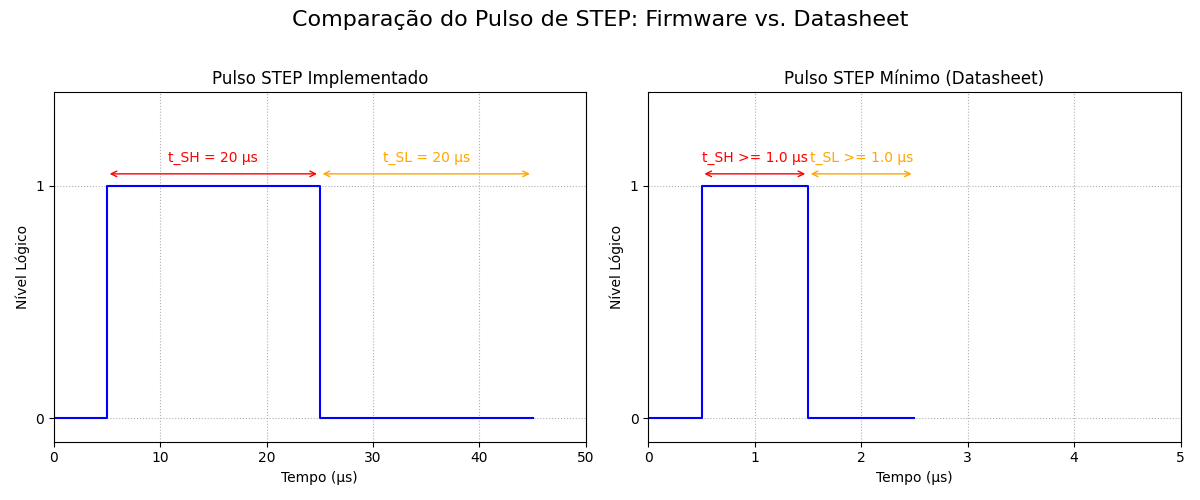
\includegraphics[width=0.88\textwidth]{figures/pdf_recovered/step_timing_tmc5160.png}
    \caption{Compara\c{c}\~ao visual entre o pulso de \texttt{STEP} implementado no firmware e o pulso m\'inimo requerido pelo TMC5160.}
    \label{fig:step-timing-tmc5160}
\end{figure}

\begin{table}[H]
    \centering
    \caption{Comparativo entre tempos m\'inimos do TMC5160 e tempos configurados no firmware.}
    \label{tab:tmc5160-timing}
    \setlength{\tabcolsep}{4pt}\footnotesize
    \begin{tabularx}{\textwidth}{lXX}
        \toprule
        Par\^ametro & Requisito do TMC5160 & Projeto \\
        \midrule
        $t_{SH}$ (alto de STEP) & $\gtrsim \SI{100}{\nano\second}$ & \SI{20}{\micro\second} \\
        $t_{SL}$ (baixo de STEP) & $\gtrsim \SI{100}{\nano\second}$ & \SI{20}{\micro\second} \\
        $t_{DSU}$ (DIR $\rightarrow$ STEP) & \SI{20}{\nano\second} & \SI{20}{\micro\second} \\
        $t_{DSH}$ (STEP $\rightarrow$ DIR) & \SI{20}{\nano\second} & \SI{20}{\micro\second} \\
        \textit{ENABLE settle} & n\~ao especificado de forma expl\'icita & \SI{40}{\micro\second} \\
        \bottomrule
    \end{tabularx}
\end{table}

Com $t_{SH} = t_{SL} = \SI{20}{\micro\second}$, o per\'iodo m\'inimo do
sinal \texttt{STEP} \'e de \SI{40}{\micro\second}, o que leva a uma taxa
f\'isica m\'axima aproximada de
\begin{equation}
    \texttt{MOTION\_MAX\_SPS}
    =
    \frac{\texttt{MOTION\_TIM6\_HZ}}
         {\texttt{MOTION\_STEP\_HIGH\_TICKS} + \texttt{MOTION\_STEP\_LOW\_TICKS}}
    =
    \frac{50000}{1 + 1}
    =
    25000~\text{steps/s}.
\end{equation}

\subsection{MicroPlyer, resolu\c{c}\~ao e \texttt{DEDGE}}

Quando \texttt{intpol=1} em \texttt{CHOPCONF}, o TMC5160 interpola cada
pulso de \texttt{STEP} at\'e 256 micropassos por meio do recurso
\emph{MicroPlyer}. Isso permite suavizar o movimento mesmo quando a
resolu\c{c}\~ao de entrada \'e mais grossa, como em configura\c{c}\~oes de
1/16 ou 1/32.

O sinal \texttt{STEP} pode ser visto como um pulso retangular de
per\'iodo $T$ e tempo em n\'ivel alto $t_{\text{alto}}$, de modo que o
\emph{duty cycle} \'e dado por
\begin{equation}
    D = \frac{t_{\text{alto}}}{T}.
\end{equation}
O bit \texttt{dedge} controla como o pulso \'e interpretado: com
\texttt{dedge=0}, apenas a borda de subida conta como passo; com
\texttt{dedge=1}, tanto a borda de subida quanto a de descida passam a
ser contabilizadas. Neste trabalho optou-se por manter \texttt{dedge=0},
com largura fixa de pulso e \emph{duty} bem controlado, o que simplifica
o \emph{timing}, evita assimetrias e reduz a sensibilidade a pequenas
varia\c{c}\~oes do sinal.

\section{DDA em Ponto Fixo (TIM6 @ 50 kHz)}
\label{sec:dda_q16}

A Figura~\ref{fig:dda-xy-simulation} ilustra o funcionamento interno do
DDA para um movimento simples de 7 passos em X e 4 passos em Y. O gr\'afico
superior mostra a evolu\c{c}\~ao dos acumuladores de fase, enquanto o
gr\'afico inferior mostra os pulsos \texttt{STEP} gerados a cada
transbordamento do acumulador.

\begin{figure}[H]
    \centering
    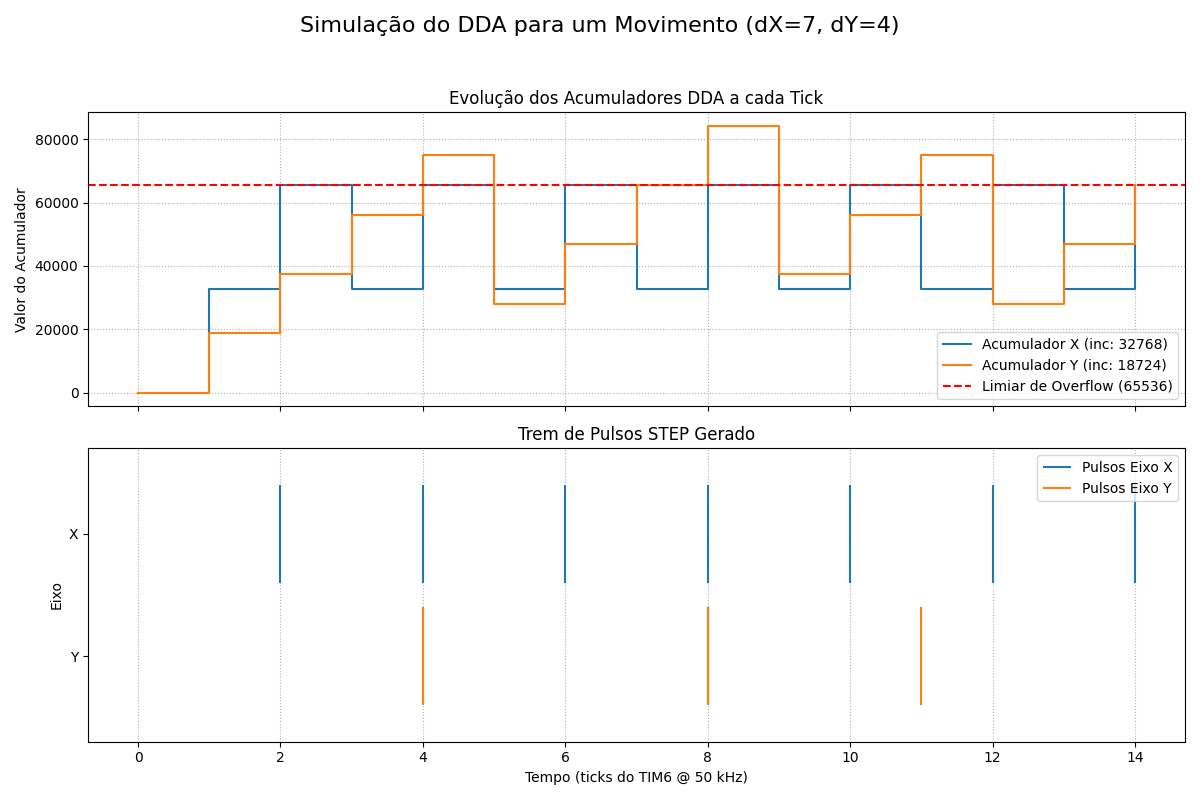
\includegraphics[width=0.88\textwidth]{figures/pdf_recovered/dda_xy_simulation.png}
    \caption{Simula\c{c}\~ao da opera\c{c}\~ao interna do DDA para um movimento de 7 passos em X e 4 em Y.}
    \label{fig:dda-xy-simulation}
\end{figure}

O gerador de passos utiliza um DDA em ponto fixo no formato Q16.16, em
que a parte inteira representa o n\'umero de passos emitidos e a parte
fracion\'aria acumula fra\c{c}\~oes de passo a cada \emph{tick}. Em
termos funcionais, o DDA atua como um integrador digital de velocidade:
a cada amostra, a refer\^encia de velocidade em \emph{steps/s} \'e
convertida em incremento de fase e, sempre que a fase acumulada cruza um
limiar unit\'ario, um novo pulso \texttt{STEP} \'e emitido. Neste texto,
\texttt{Q16\_1} denota exatamente esse limiar de um passo inteiro
representado no formato Q16.16.

Para cada eixo $i$, o firmware mant\'em os seguintes estados:
\begin{itemize}
\item \texttt{dda\_accum\_q16}, que guarda a fase acumulada em formato
  Q16.16;
\item \texttt{dda\_inc\_q16}, proporcional \`a velocidade efetiva;
\item \texttt{v\_actual\_sps}, velocidade efetiva em \emph{steps/s},
  atualizada a cada \SI{1}{\milli\second} pelo TIM7;
\item \texttt{step\_high} e \texttt{step\_low}, contadores que garantem
  largura de pulso e espa\c{c}amento m\'inimo entre pulsos.
\end{itemize}

A integra\c{c}\~ao da velocidade em fase fracion\'aria segue
\begin{equation}
    \texttt{dda\_accum\_q16}
    \leftarrow
    \texttt{dda\_accum\_q16}
    +
    \texttt{dda\_inc\_q16}.
\end{equation}
Sempre que o acumulador ultrapassa um passo inteiro em Q16.16,
considera-se que mais um pulso deve ser emitido. O incremento do DDA \'e
calculado diretamente a partir da velocidade efetiva desejada:
\begin{equation}
    \texttt{dda\_inc\_q16}
    =
    Q16\!\left(
        \frac{\texttt{v\_actual\_sps}}
             {\texttt{MOTION\_TIM6\_HZ}}
    \right).
\end{equation}
Intuitivamente, isso significa que, em m\'edia, a taxa de cruzamentos do
acumulador equivale \`a velocidade desejada em \emph{steps/s}.

\begin{algorithm}[H]
    \caption{Atualiza\c{c}\~ao do DDA Q16.16 no TIM6 (por eixo).}
    \label{alg:dda-tick}
    \begin{algorithmic}[1]
        \Procedure{dda\_tick}{axis}
            \If{\texttt{step\_high} $> 0$}
                \State decrementa \texttt{step\_high}
                \If{\texttt{step\_high} $= 0$}
                    \State \texttt{motion\_hw\_step\_low(axis)}
                    \State \texttt{step\_low} $\gets$ \texttt{MOTION\_STEP\_LOW\_TICKS}
                \EndIf
                \State \Return
            \EndIf
            \If{\texttt{step\_low} $> 0$}
                \State decrementa \texttt{step\_low}
                \State \Return
            \EndIf
            \If{\texttt{emitted\_steps} $\ge$ \texttt{total\_steps}}
                \State \Return
            \EndIf
            \If{\texttt{en\_settle\_ticks} $> 0$ \textbf{or} \texttt{dir\_settle\_ticks} $> 0$}
                \State decrementa os contadores de guarda ainda ativos
                \State \Return
            \EndIf
            \State \texttt{dda\_accum\_q16} $\gets$ \texttt{dda\_accum\_q16} + \texttt{dda\_inc\_q16}
            \If{\texttt{dda\_accum\_q16} $\ge$ \texttt{Q16\_1}}
                \State \texttt{dda\_accum\_q16} $\gets$ \texttt{dda\_accum\_q16} - \texttt{Q16\_1}
                \State \texttt{motion\_hw\_step\_high(axis)}
                \State \texttt{step\_high} $\gets$ \texttt{MOTION\_STEP\_HIGH\_TICKS}
                \State \texttt{emitted\_steps} $\gets$ \texttt{emitted\_steps} + 1
            \EndIf
        \EndProcedure
    \end{algorithmic}
\end{algorithm}

\section{Rampa Trapezoidal (TIM7 @ 1 kHz)}
\label{sec:rampa_trapezoidal}

A cada \SI{1}{\milli\second}, o TIM7 atualiza a velocidade alvo de cada
eixo e aplica uma rampa trapezoidal de acelera\c{c}\~ao ou
desacelera\c{c}\~ao. A refer\^encia de velocidade em \emph{steps/s} \'e
obtida a partir da quantidade de passos por amostra configurada pelo
host:
\begin{equation}
    v_{\text{cmd,sps}} = \texttt{velocity\_per\_tick} \times 1000.
\end{equation}

A dist\^ancia de frenagem em passos \'e calculada por
\begin{equation}
    s_{\text{brake}} =
    \left\lfloor \frac{v^2}{2a} \right\rfloor,
    \qquad
    v = \texttt{v\_actual\_sps},
    \quad
    a = \texttt{accel\_sps2}.
\end{equation}
O operador piso $\lfloor \cdot \rfloor$ indica que a express\~ao \'e
convertida para um n\'umero inteiro de passos. Esse termo representa o
n\'umero de passos necess\'arios para reduzir a
velocidade atual a zero com acelera\c{c}\~ao constante. Em cada ciclo do
TIM7, a l\'ogica de rampa segue tr\^es passos:
\begin{enumerate}
\item se os passos remanescentes forem menores ou iguais a
  $s_{\text{brake}}$, inicia-se a frenagem;
\item caso contr\'ario, a velocidade acelera em dire\c{c}\~ao a
  $v_{\text{cmd,sps}}$, respeitando o limite
  \texttt{MOTION\_MAX\_SPS};
\item ao final, recalcula-se \texttt{dda\_inc\_q16} para que o DDA reflita
  a nova velocidade de alvo.
\end{enumerate}

\begin{algorithm}[H]
    \caption{Atualiza\c{c}\~ao da rampa trapezoidal no TIM7 (por eixo).}
    \label{alg:rampa-tim7}
    \begin{algorithmic}[1]
        \Procedure{update\_ramp}{$v, v_{\text{cmd}}, a, rem$}
            \State $T_s \gets \SI{1}{\milli\second}$
            \State $s_{\text{brake}} \gets \left\lfloor \frac{v^2}{2a} \right\rfloor$
            \If{$rem \le s_{\text{brake}}$}
                \State $v \gets \max(0, v - aT_s)$
            \Else
                \State $v \gets v + aT_s$
                \State $v \gets \min(v, v_{\text{cmd}}, \texttt{MOTION\_MAX\_SPS})$
            \EndIf
            \State \texttt{v\_actual\_sps} $\gets v$
            \State \texttt{dda\_inc\_q16} $\gets Q16(v/\texttt{MOTION\_TIM6\_HZ})$
            \State \Return \texttt{v\_actual\_sps}, \texttt{dda\_inc\_q16}
        \EndProcedure
    \end{algorithmic}
\end{algorithm}

A Figura~\ref{fig:rampa-trapezoidal-simulada} apresenta um perfil de
velocidade simulado a partir dos par\^ametros do firmware. O gr\'afico
ajuda a visualizar a transi\c{c}\~ao entre acelera\c{c}\~ao, velocidade de
cruzeiro e frenagem, complementando o pseudoc\'odigo do
Algoritmo~\ref{alg:rampa-tim7}.

\begin{figure}[H]
    \centering
    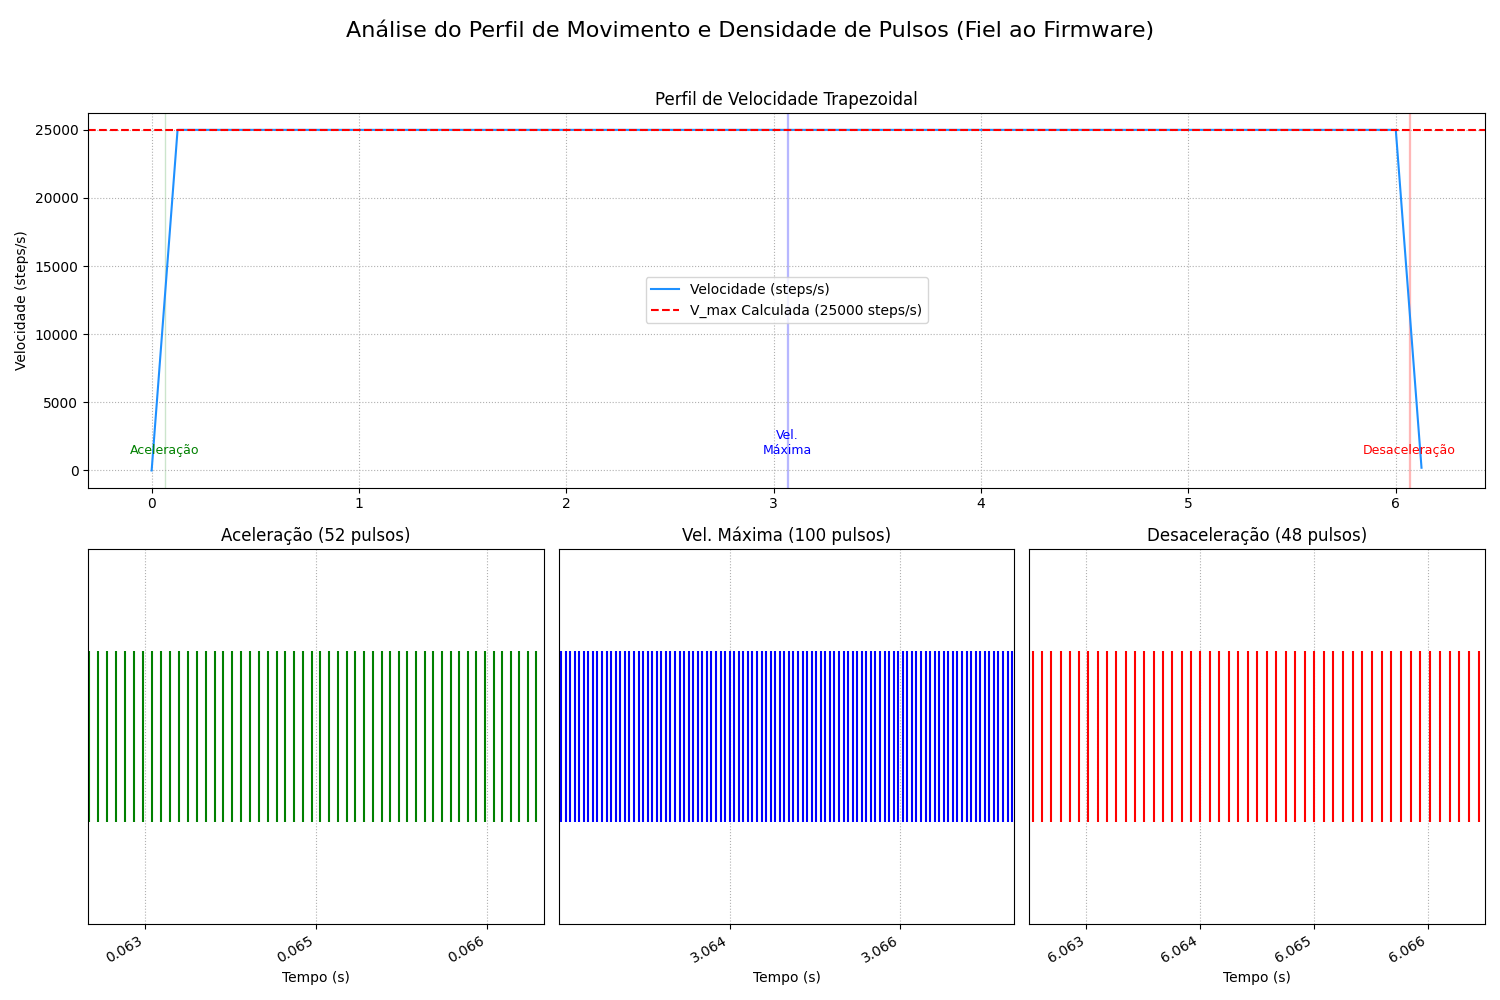
\includegraphics[width=0.86\textwidth]{figures/pdf_recovered/trapezoidal_ramp_simulation.png}
    \caption{Perfil de velocidade da rampa trapezoidal simulado a partir dos par\^ametros do firmware.}
    \label{fig:rampa-trapezoidal-simulada}
\end{figure}

O projeto manteve, nos ensaios relatados neste trabalho, o valor
\texttt{DEMO\_ACCEL\_SPS2 = 200000} como acelera\c{c}\~ao padr\~ao,
podendo ser ajustado por eixo. A fun\c{c}\~ao de passos remanescentes
soma o segmento ativo com os segmentos ainda enfileirados, permitindo que
a decis\~ao de frenagem leve em conta todo o trecho pendente.

\section{Controle PI de Posi\c{c}\~ao com Encoder}
\label{sec:pi_encoder}

O erro posicional em passos DDA \'e calculado pela diferen\c{c}a entre o
alvo acumulado e a posi\c{c}\~ao medida pelo encoder, convertida para a
mesma unidade:
\begin{equation}
    e =
    \texttt{target\_steps}
    -
    \left\lfloor
        \texttt{enc\_rel}
        \cdot
        \frac{\texttt{DDA\_STEPS\_PER\_REV}}
             {\texttt{ENC\_COUNTS\_PER\_REV}}
    \right\rfloor.
\end{equation}
Neste trabalho, \texttt{DDA\_STEPS\_PER\_REV} \'e calculado a partir de
400 passos por volta do motor de $0{,}9^\circ$ multiplicados pelo fator
de microstepping, enquanto \texttt{ENC\_COUNTS\_PER\_REV} depende do
encoder configurado em cada eixo.

Aplica-se uma zona morta de
$\pm \texttt{MOTION\_PI\_DEADBAND\_STEPS}$ para evitar que ru\'ido de
quantiza\c{c}\~ao e pequenas oscila\c{c}\~oes mec\^anicas realimentem o
controlador em torno do alvo. Para o termo derivativo, utiliza-se um
filtro exponencial discreto:
\begin{equation}
    d[n]
    \leftarrow
    d[n-1] + \frac{\Delta e - d[n-1]}{2^\alpha},
    \qquad
    \alpha = 8.
\end{equation}

Os ganhos $k_p$, $k_i$ e $k_d$ s\~ao representados como inteiros de
16 bits, com sa\'ida escalada por $2^{-8}$:
\begin{equation}
    \Delta v =
    \frac{k_p e + k_i P_e + k_d d}{2^8},
\end{equation}
com \emph{anti-windup} por limita\c{c}\~ao da integral em
$\pm \texttt{MOTION\_PI\_I\_CLAMP}$ e satura\c{c}\~ao sim\'etrica em
$\pm \texttt{MOTION\_MAX\_SPS}$. A corre\c{c}\~ao ajusta a velocidade de
refer\^encia antes da rampa trapezoidal, preservando os limites f\'isicos
do movimento.

\section{Fila de Movimentos e Segmenta\c{c}\~ao}
\label{sec:fila_segmentacao}

O protocolo do host enfileira segmentos de movimento com deslocamentos
$S=(s_x, s_y, s_z)$ e velocidades-base
$V=(v_x, v_y, v_z)$. No in\'icio de cada trecho, o firmware zera os
acumuladores do DDA, aplica guardas de \texttt{ENABLE} e \texttt{DIR},
inicializa as velocidades-alvo por eixo e habilita a sa\'ida apenas se o
total de passos daquele eixo for maior do que zero.

A transi\c{c}\~ao para o pr\'oximo segmento acontece quando todos os
eixos terminam o trecho corrente, isto \'e, quando
\texttt{emitted\_steps == total\_steps} para todos os eixos e nenhum
pino \texttt{STEP} permanece em n\'ivel alto. Esse mecanismo evita a
troca de segmento no meio de um pulso e impede inconsist\^encias entre a
fila de comando e o estado eletromec\^anico do conjunto.

\section{Mapeamento para o TMC5160}
\label{sec:mapeamento_tmc5160}

\subsection{Gera\c{c}\~ao de STEP/DIR}

Em modo \texttt{STEP}/\texttt{DIR}, o backend de GPIO implementa quatro
garantias b\'asicas para o TMC5160:
\begin{enumerate}
\item largura fixa de \texttt{STEP} por meio de \texttt{step\_high};
\item intervalo m\'inimo em n\'ivel baixo por meio de \texttt{step\_low};
\item tempo de \emph{setup} de \texttt{DIR} antes do primeiro pulso do
  trecho;
\item \emph{settle} de \texttt{ENABLE} antes do in\'icio da emiss\~ao.
\end{enumerate}
Com isso, o sinal \texttt{STEP} opera com \emph{duty} pr\'oximo de 50\%
em regime e permanece compat\'ivel com os tempos m\'inimos exigidos pelo
driver.

\subsection{Resolu\c{c}\~ao de microstepping e MicroPlyer}

O host pode ajustar \texttt{MICROSTEP\_FACTOR} quando o sistema est\'a
parado. Quando \texttt{intpol=1} no TMC5160, a resolu\c{c}\~ao efetiva de
corrente nas bobinas pode ser maior do que a resolu\c{c}\~ao do sinal
\texttt{STEP}, o que favorece a suavidade do movimento mesmo sem elevar a
frequ\^encia de pulsos para valores extremos.

\section{Par\^ametros-chave do Projeto}
\label{sec:parametros_projeto}

\begin{table}[H]
    \centering
    \caption{Par\^ametros de tempo e limites usados no firmware.}
    \label{tab:parametros-firmware}
    \setlength{\tabcolsep}{4pt}\footnotesize
    \begin{tabularx}{\textwidth}{lXl}
        \toprule
        Par\^ametro & Significado & Valor de teste \\
        \midrule
        \texttt{MOTION\_TIM6\_HZ} & Frequ\^encia do la\c{c}o de DDA/\texttt{STEP} & \SI{50}{\kilo\hertz} \\
        \texttt{MOTION\_STEP\_HIGH\_TICKS} & Largura alta do \texttt{STEP} & 1 \emph{tick} = \SI{20}{\micro\second} \\
        \texttt{MOTION\_STEP\_LOW\_TICKS} & Baixo m\'inimo entre pulsos & 1 \emph{tick} = \SI{20}{\micro\second} \\
        \texttt{MOTION\_DIR\_SETUP\_TICKS} & \emph{Setup} de \texttt{DIR} antes do \texttt{STEP} & 1 \emph{tick} = \SI{20}{\micro\second} \\
        \texttt{MOTION\_ENABLE\_SETTLE\_TICKS} & Tempo ap\'os \texttt{ENABLE} & 2 \emph{ticks} = \SI{40}{\micro\second} \\
        \texttt{MOTION\_MAX\_SPS} & Limite f\'isico de velocidade & 25 kSPS \\
        \texttt{MOTION\_PI\_DEADBAND\_STEPS} & Zona morta do PI & 10 passos \\
        \texttt{MOTION\_PI\_I\_CLAMP} & Limite da integral & $\pm 200000$ \\
        \texttt{kd\_alpha\_bits} & Filtro exponencial na derivada & 8 \\
        \bottomrule
    \end{tabularx}
\end{table}

\section{Coordena\c{c}\~ao Multi-eixos}
\label{sec:coordenacao_multi_eixos}

O firmware adota uma coordena\c{c}\~ao baseada no progresso relativo dos
eixos. Cada eixo acompanha o quanto j\'a percorreu do segmento ativo em
rela\c{c}\~ao ao alvo total, e o eixo mestre \'e definido como aquele com
menor fra\c{c}\~ao de avan\c{c}o:
\begin{equation}
    i^\ast = \argmin_i \frac{\texttt{emitted\_steps}_i}{\texttt{total\_steps}_i}.
\end{equation}

Com o mestre definido, duas pol\'iticas principais s\~ao aplicadas:
\begin{enumerate}
\item \textbf{Rampa guiada pelo mestre}: a decis\~ao de frenagem usa o
  restante global do mestre, alinhando a desacelera\c{c}\~ao entre os
  eixos.
\item \textbf{T\'ermino por mestre}: o movimento s\'o \'e conclu\'ido
  quando o mestre alcan\c{c}a o restante nulo, evitando que um eixo ainda
  atrasado seja abandonado.
\end{enumerate}

\noindent Em termos pr\'aticos, isso significa que a decis\~ao de frear
ou de manter acelera\c{c}\~ao deixa de olhar apenas o restante local de
cada eixo e passa a considerar o eixo mais atrasado como refer\^encia de
sincronismo do grupo.

\begin{algorithm}[H]
    \caption{Sele\c{c}\~ao do eixo mestre e coordena\c{c}\~ao de remanescentes.}
    \label{alg:eixo-mestre}
    \begin{algorithmic}[1]
        \Procedure{update\_master\_and\_rem}{total\_steps[], emitted\_steps[]}
            \State $m \gets 0$
            \State $p_{\min} \gets 1.0$
            \For{$i \gets 0$ at\'e $\texttt{MOTION\_AXIS\_COUNT}-1$}
                \If{$\texttt{total\_steps}[i] > 0$}
                    \State $p_i \gets \texttt{emitted\_steps}[i] / \texttt{total\_steps}[i]$
                    \If{$p_i < p_{\min}$}
                        \State $p_{\min} \gets p_i$
                        \State $m \gets i$
                    \EndIf
                \EndIf
            \EndFor
            \State \texttt{master\_axis} $\gets m$
            \State \texttt{rem\_master} $\gets$ restante global do eixo $m$
            \For{$i \gets 0$ at\'e $\texttt{MOTION\_AXIS\_COUNT}-1$}
                \State \texttt{rem\_steps}[i] $\gets$ \texttt{rem\_master}
            \EndFor
            \State \Return \texttt{master\_axis}, \texttt{rem\_steps[]}
        \EndProcedure
    \end{algorithmic}
\end{algorithm}

\section{Simulador Interativo em Python}
\label{sec:simulador_python}

Para validar rapidamente pol\'iticas de sincronismo, curvas de rampa e o
impacto do limitador por erro entre eixos, foi desenvolvido um simulador
interativo em Python. A aplica\c{c}\~ao reproduz os blocos l\'ogicos do
firmware e adota as mesmas constantes principais do projeto:
amostragem de controle a \SI{1}{\kilo\hertz}, gera\c{c}\~ao de passos pelo
DDA a \SI{50}{\kilo\hertz} e ganhos inteiros escalados por
\texttt{K\_SCALE = 256}.

Do ponto de vista do usu\'ario, a interface permite configurar, por eixo:
(i) o deslocamento alvo em passos; (ii) a velocidade nominal em
\emph{steps/s}; (iii) o sentido do movimento; e
(iv) os ganhos $K_p$, $K_i$ e $K_d$. Um painel adicional aplica carga de
atrito program\'avel com amplitude e janela temporal por eixo, viabilizando
cen\'arios de teste com cargas desiguais.

A Figura~\ref{fig:simulador-python} mostra um cen\'ario de simula\c{c}\~ao
com atrito program\'avel por eixo. A interface permite observar, no mesmo
ensaio, as curvas de posi\c{c}\~ao, velocidade, erro de sincronismo,
janelas de carga e indicadores de desempenho.

\begin{figure}[H]
    \centering
    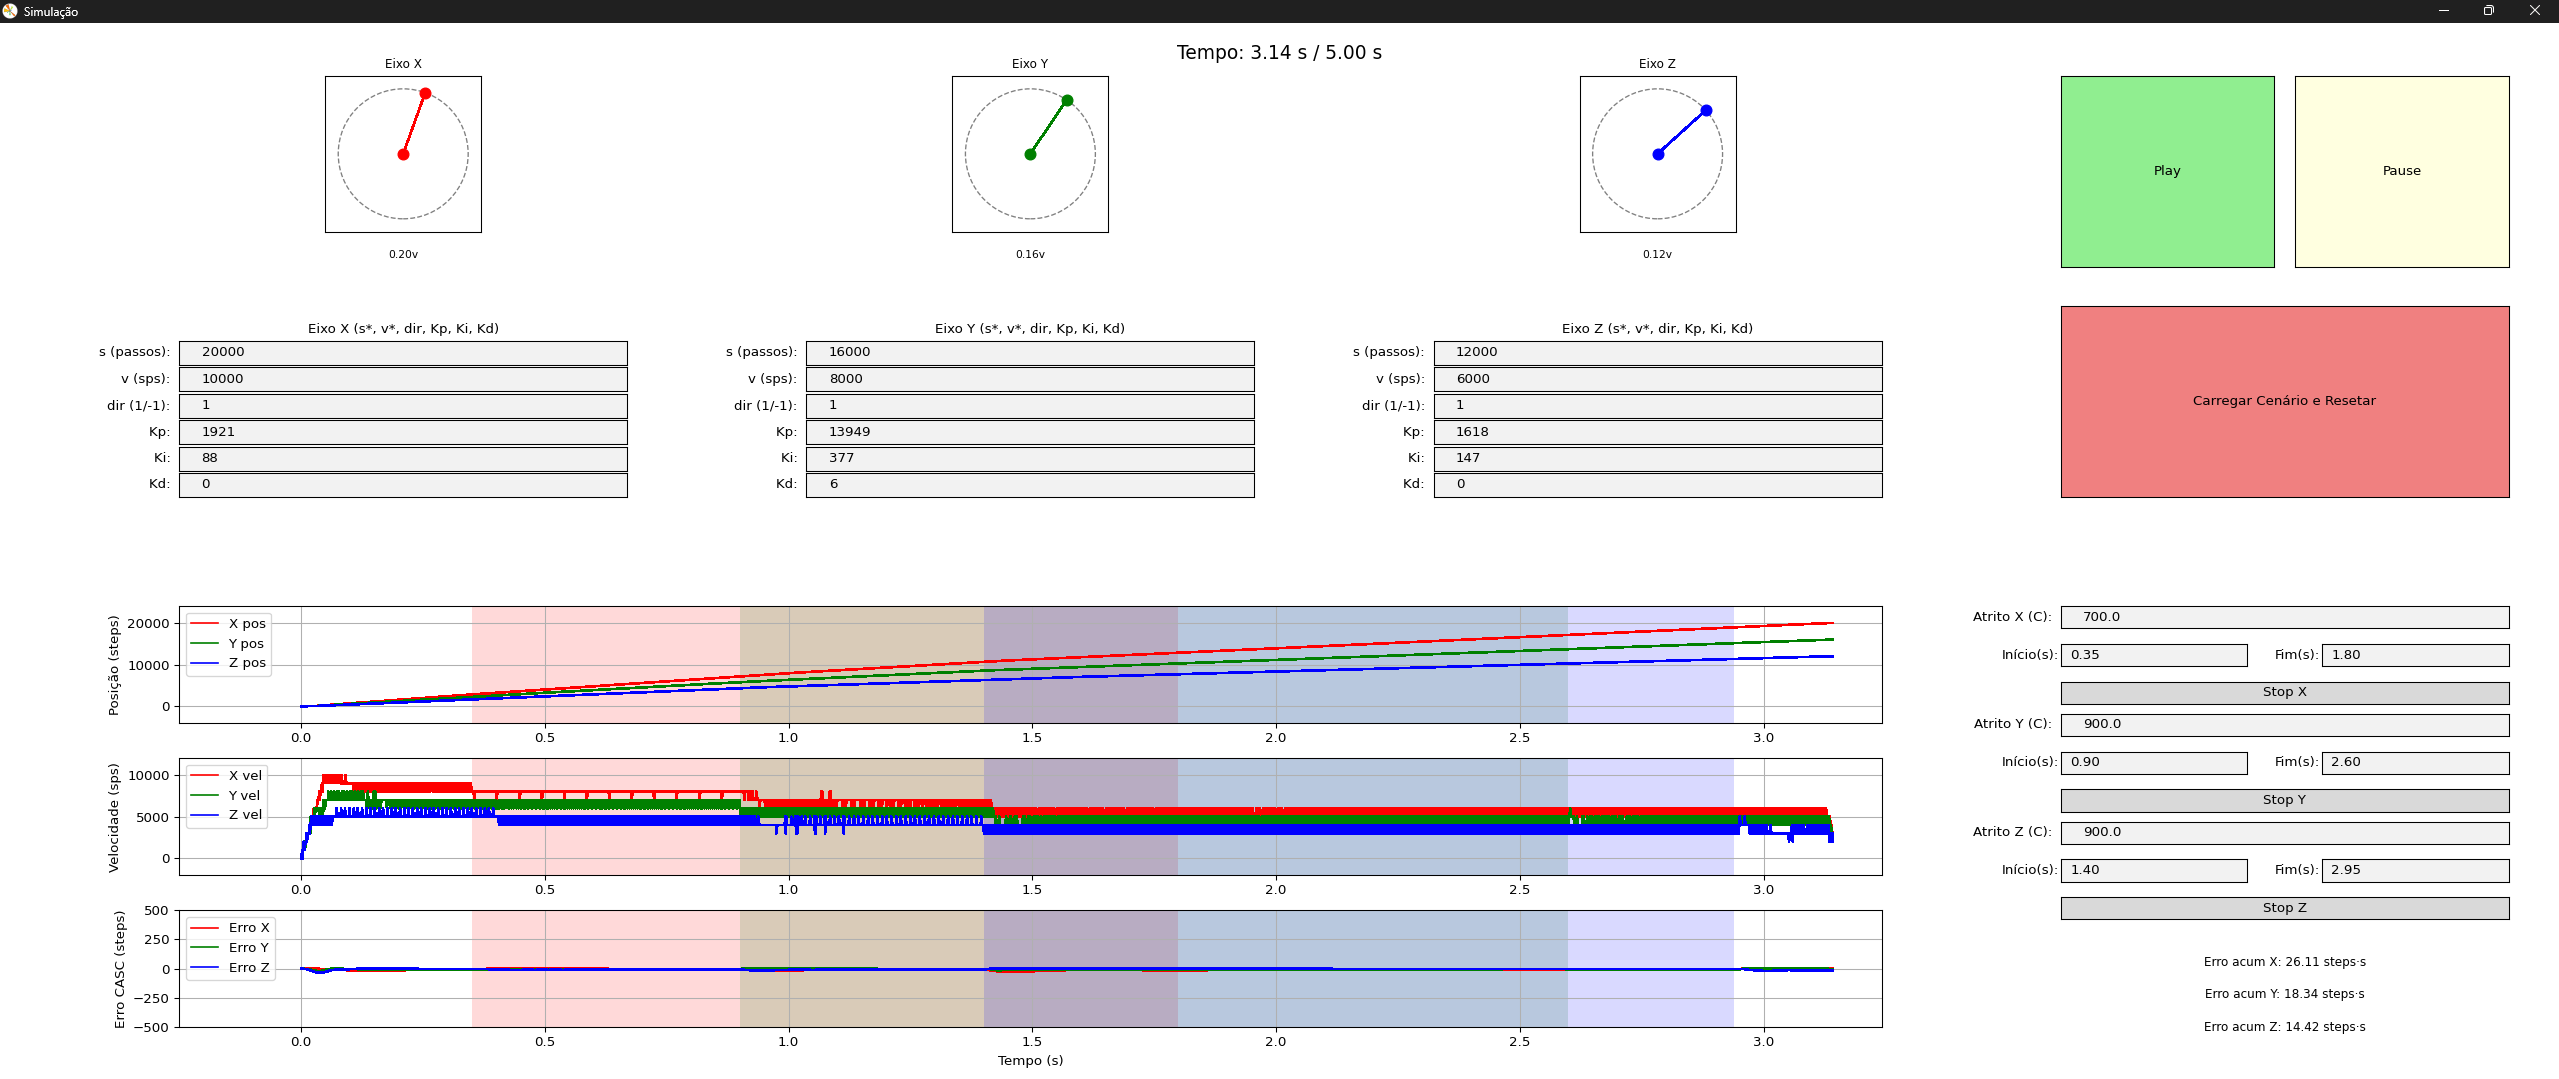
\includegraphics[width=0.95\textwidth]{figures/pdf_recovered/python_interactive_simulator.png}
    \caption{Cen\'ario de simula\c{c}\~ao com atrito program\'avel por eixo, destacando janelas de carga e impacto sobre posi\c{c}\~ao, velocidade e erro de sincronismo.}
    \label{fig:simulador-python}
\end{figure}

O la\c{c}o principal do simulador executa, a cada
$T_s = \SI{1}{\milli\second}$:
\begin{enumerate}
\item ativa a carga program\'avel e combina um termo viscoso;
\item elege o eixo mestre e sincroniza os alvos proporcionais dos demais;
\item calcula o erro de posi\c{c}\~ao em passos DDA;
\item aplica um PI(D) digital inteiro com \emph{deadband},
  \emph{anti-windup} e derivada filtrada;
\item executa a rampa trapezoidal;
\item integra a velocidade final com o DDA a \SI{50}{\kilo\hertz};
\item converte as contagens de encoder para passos DDA e fecha o la\c{c}o
  de realimenta\c{c}\~ao;
\item encerra quando todos os eixos ativos entram na janela de
  toler\^ancia.
\end{enumerate}

Os gr\'aficos exibem posi\c{c}\~ao, velocidade e erro de sincronismo, al\'em
de indicadores textuais do erro acumulado por eixo (IAE, em
\emph{steps}$\cdot$s) e da carga ativa. Um modo \emph{headless} permite
executar a simula\c{c}\~ao e gravar CSVs sem abrir a interface gr\'afica.

\section{Boas pr\'aticas e Diagn\'ostico}
\label{sec:boas_praticas_diag}

Para minimizar \emph{glitches} em \texttt{STEP}/\texttt{DIR} e evitar
condi\c{c}\~oes indevidas no TMC5160, a sequ\^encia recomendada por
segmento de movimento \'e: (i) ajustar \texttt{DIR};
(ii) aguardar o tempo de \emph{setup};
(iii) habilitar o driver com \texttt{EN};
(iv) aguardar o \emph{settle} de habilita\c{c}\~ao; e
(v) somente ent\~ao iniciar a emiss\~ao de pulsos \texttt{STEP}.

O la\c{c}o de alta frequ\^encia do TIM6 permanece dedicado ao DDA e ao
controle da largura dos pulsos, enquanto c\'alculos mais custosos, como
PI, rampa e telemetria, s\~ao executados no TIM7 a
\SI{1}{\kilo\hertz}. Para preservar essa separa\c{c}\~ao, recomenda-se
evitar chamadas de depura\c{c}\~ao dentro da ISR do TIM6 e deslocar logs
para a USART ou para o caminho de observabilidade do host.

As requisi\c{c}\~oes de estado de encoder e de origem exp\~oem, via USART
e SPI, informa\c{c}\~oes essenciais para diagn\'ostico: posi\c{c}\~ao
absoluta e relativa por eixo, erro instant\^aneo do PI, refer\^encia de
zero e indicadores de estol. A an\'alise conjunta desses sinais com logs
de tempo, posi\c{c}\~ao e velocidade permite identificar folgas, erro
acumulado e desbalanceamento de carga entre eixos.

Mesmo com ampla margem em rela\c{c}\~ao aos tempos de \emph{setup} e
\emph{hold} do TMC5160, boas pr\'aticas adicionais incluem: manter o
\emph{duty} de \texttt{STEP} pr\'oximo de 50\% quando \texttt{dedge=1},
garantir bordas limpas e revisar periodicamente registros como
\texttt{GSTAT} e \texttt{DRV\_STATUS} em busca de alertas de temperatura,
subtens\~ao e erro de \emph{driver}.
